\section{Network Methodology}
In this section there is a technical description of the methodology used to create and analyze the network.

\subsection{Network Creation}
In this project, a bipartite graph was created where nodes represent symptoms (lightcoral) and diseases (lightblue),
and edges denote the presence of symptoms in diseases.
For simplicity, the graph is unweighted, and all edges have a weight of 1.
Prior to graph creation, a preliminary data analysis was conducted to identify isolated nodes.
Additionally, an analysis of the node degree distribution was performed to assess whether the distribution follows a power law (see Section 5.1).\\
The analysis revealed the presence of several symptoms, precisely 52 out of 377, not associated with any disease.
Consequently, these isolated symptoms were removed from the graph as they do not contribute informative content.
Diseases without associated symptoms were also removed for the same reason.\\
Figure \ref{fig:bipartite_graph} illustrates the resulting bipartite graph. As observed, diseases tend to be peripheral,
while symptoms tend to be central. This observation arises from the fact that symptoms are shared by multiple diseases,
whereas diseases exhibit distinct symptoms. Furthermore, symptoms are fewer in number than diseases,
making it more likely for a symptom to be shared among multiple diseases.\\
Figure \ref{fig:unipartite_graphs} presents the unipartite graphs of symptoms and diseases.
\begin{figure*}[thbp]
    \centering
    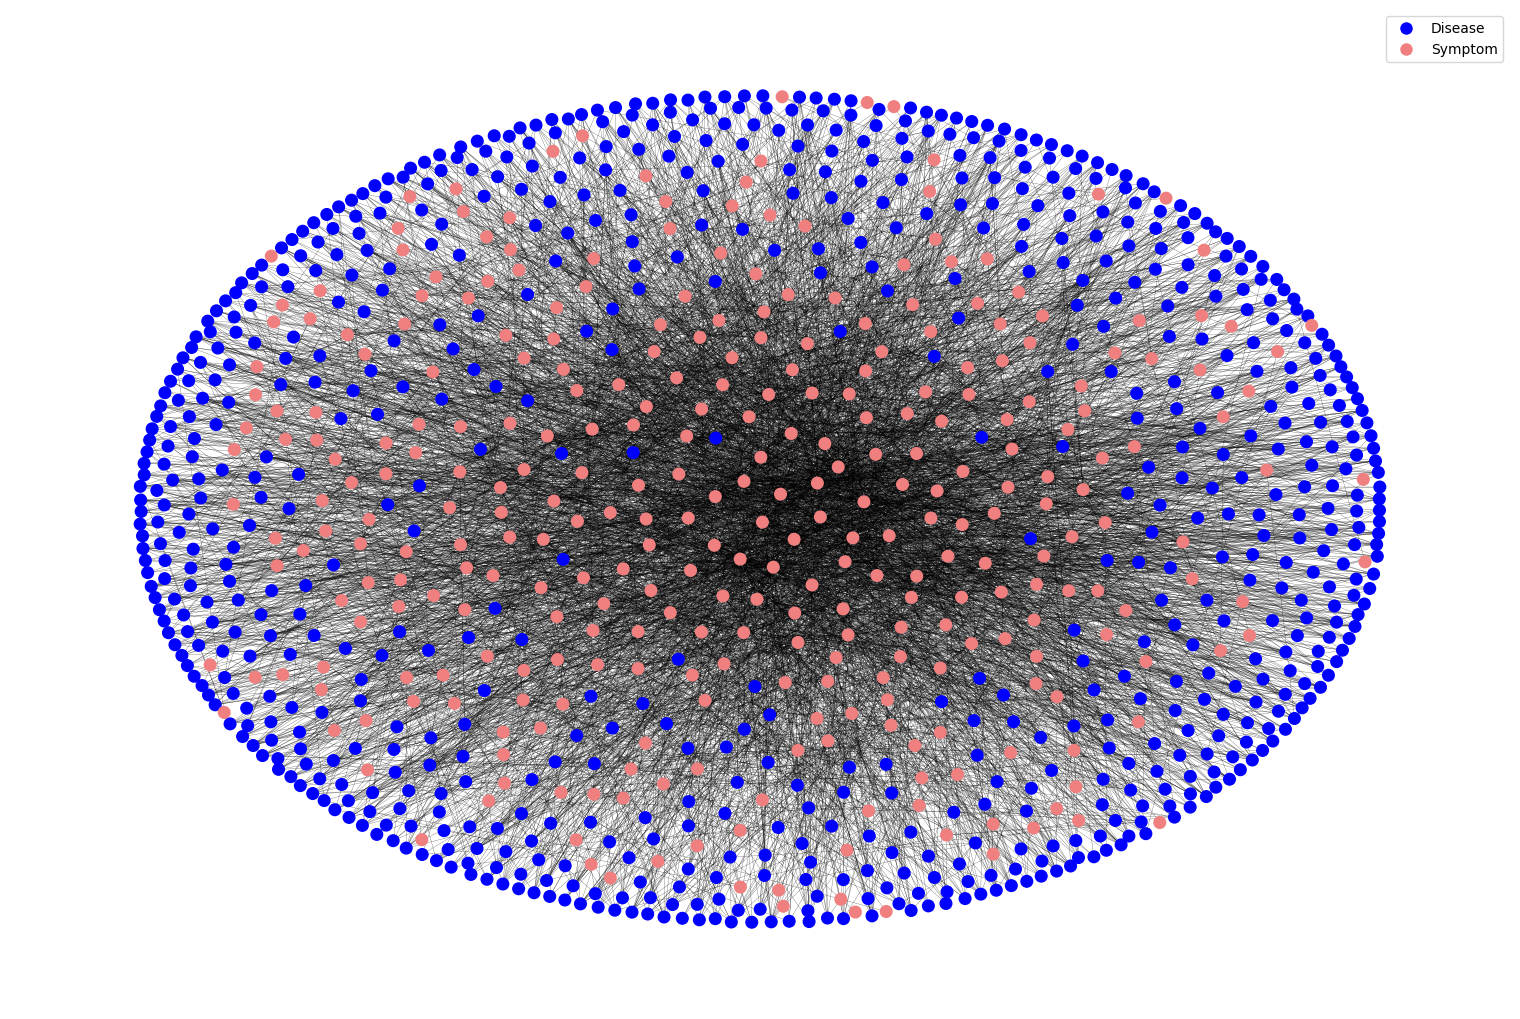
\includegraphics[width=.9\textwidth]{network.png}
    \caption{Visual representation of the symptom-disease bipartite graph.}
    \label{fig:bipartite_graph}
\end{figure*}
\noindent

\begin{figure}[H]
    \centering
    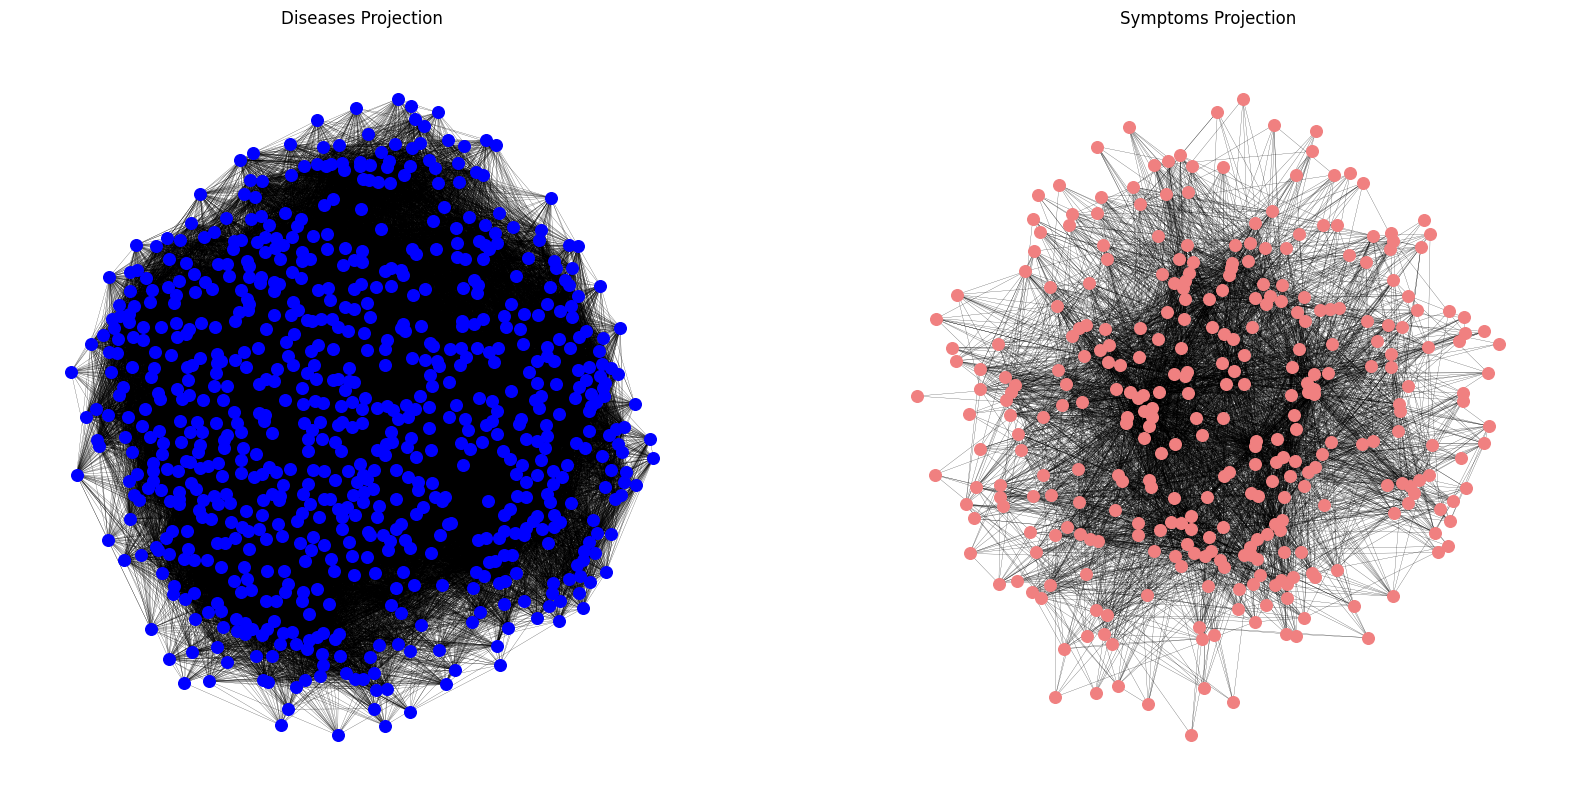
\includegraphics[width=\columnwidth]{unipartite_networks.png}
    \caption{Visual representation of symptom and disease unipartite graphs.}
    \label{fig:unipartite_graphs}
\end{figure}
\noindent

\subsection{Method of Reflections}

To identify influential nodes in the symptom-disease network, we introduce two indices that capture the relative importance of each actor.
The first index, referred to as the Symptom Influence (\textit{SI}) index, not only ranks symptom nodes based on their frequency (level-1)
but also considers whether a symptom is present in diseases affected by numerous other symptoms (level-2) or in diseases affected by only a few symptoms.\\
Conversely, the second index, known as the Disease Influence (\textit{DI}) index,
assesses the distinct symptoms related to a disease (level-1) and whether a disease exhibits symptoms that affect many other diseases (level-2).\\
In other words, level-1 of these indices quantifies the number of symptoms associated with a disease,
while level-2 measures the interconnectedness and broader impact of symptoms or diseases within the network.
For the Symptom Influence (\textit{SI}) index, level-2 takes into account the presence of a symptom across diseases,
shedding light on whether a particular symptom tends to co-occur with a wide range of other symptoms or is more specific to a subset of diseases.
This dual-level analysis provides a nuanced understanding of the significance of symptoms based not only on their individual prevalence (level-1)
but also on their associations with other symptoms across different diseases (level-2). Similarly, for the Disease Influence (\textit{DI}) index,
level-2 assesses the extent to which a disease's symptoms have ripple effects on other diseases, indicating the potential for cascading impacts within the network.\\
We adapt the level-\textit{N} indices following the approach of \citeauthor{Hidalgo_2007},\cite{Hidalgo_2007} and  \citeauthor{Hidalgo_2009},\cite{Hidalgo_2009}.
The level-\textit{N} indices are defined as:
\begin{equation}
    SI_{v, N} = \frac{1}{SI_{v, 1}} \sum_u W(v, u) DI_{u, N-1}
\end{equation}
\begin{equation}
    DI_{u, N} = \frac{1}{DI_{u, 1}} \sum_v W(v, u) SI_{v, N-1}
\end{equation}
\noindent
Here, $SI_{v, 1}$ and $DI_{u, 1}$ represent the level-1 indices, and $W(v,u)$ denotes the edge weight between symptom $v$ and disease $u$.
The level-1 indices are defined as follows:
\begin{equation}
    SI_{v, 1} = \sum_u W(v, u)
\end{equation}
\begin{equation}
    DI_{u, 1} = \sum_v W(v, u)
\end{equation}
\noindent
Since our network is not weighted ($W(v,u)=1$ if symptom $v$ is associated with disease $u$ and $W(v,u)=0$ otherwise),
$SI_{v,1}$ and $DI_{u,1}$ are equal to the degree of symptom $v$ and disease $u$, respectively.
\subsubsection*{Statistical Validation of SI and DI}

In our effort to identify significant nodes within the symptom-disease network,
we focus on discerning topological properties that hold statistical significance.
Our goal is to differentiate higher-order properties that are directly associated with local node features from those
that emerge from the intricate interactions among nodes.\\
Relevant studies by \citeauthor{Squartini_2011_a} \cite{Squartini_2011_a, Squartini_2011_b} and \citeauthor{Spelta_2023} \cite{Spelta_2023}
highlight how higher-order network properties naturally capture structured group interactions.
Here, a 'group' is defined as all players connected by a 'hyperlink,' representing the higher-order analog of a link.\\
The sampling of random graphs with specified properties plays a pivotal role in network analysis,
serving as fundamental null models for identifying patterns, including communities and motifs.\\
To statistically assess the significance of SI and DI, we adopt a hypothesis testing approach based on a null model.
Specifically, we posit \textbf{H0} as the hypothesis that SI and DI level-2 do not offer additional information compared to level-1,
and \textbf{H1} as the opposite.
To test these hypotheses, we generate 5000 random networks using a null model with the same level-1 properties as the original network.\\
With this ample set of null models, we assume that the distribution of SI and DI is Gaussian, leveraging the Central Limit Theorem (CLT).
For each null model, we calculate the mean ($\mu$) and standard deviation ($\sigma$) of SI and DI and compute the z-score for each SI and DI level-2,
as expressed in the following equation:

\begin{equation}
    z_{SI_{v, 2}} = \frac{SI_{v, 2} - \mu_{SI_{v, 2}}}{\sigma_{SI_{v, 2}}}
\end{equation}
\noindent
If \textbf{H0} holds true,the z-scores of SI and DI should be normally distributed with a mean of 0 and a standard deviation of 1.
Conversely, if \textbf{H1} is true, the z-scores of SI and DI should be normally distributed with a mean and standard deviation different from 0 and 1,
respectively.


% ------------------- Betweenness -------------------

\subsection{Betweenness Centrality}
The betweenness centrality of a node \(v\), as defined by \Citeauthor{Brandes_2008} \cite{Brandes_2008},
is calculated as the sum of the fraction of all-pairs shortest paths that pass through \(v\):

\begin{equation}
    c_B(v) = \sum_{s,t \in V} \frac{\sigma(s, t|v)}{\sigma(s, t)} \label{eq:betweenness}
\end{equation}
\noindent
where:

\begin{itemize}
    \setlength\itemsep{0.4em} % set space between items
    \item \(V\): The set of nodes.
    \item \(\sigma(s, t)\): The number of shortest paths from node \(s\) to node \(t\).
    \item \(\sigma(s, t|v)\): The number of those shortest paths from node \(s\) to node \(t\) that pass
          through some node \(v\) other than \(s\) and \(t\).
    \item If \(s = t\), then \(\sigma(s, t) = 1\).
    \item If \(v \in \{s, t\}\), then \(\sigma(s, t|v) = 0\).
\end{itemize}
\noindent
To compute the betweenness centrality, the NetworkX function \textit{nx.bipartite.betweenness\_centrality}
was utilized. This function implements the algorithm proposed by \Citeauthor{Brandes_2004} \cite{Brandes_2004},
specifically designed for bipartite graphs, and includes proper normalization for accurate results.

% ------------------- Communities Detection -------------------
\subsection{Communities Detection}
Prior to applying any community detection algorithm, two crucial steps must be performed:\\


\begin{itemize}
    \setlength\itemsep{1em} % set space between items
    \item \textbf{Graph Projections:} The bipartite graph needs to be projected into two separate graphs,
          one for each set of nodes. In our case, the two sets represent symptoms and diseases. To achieve this,
          the NetworkX function \textit{nx.bipartite.projected\_graph} is employed, returning the projection of
          the bipartite graph onto the specified nodes.

    \item \textbf{Compute Similarity:} The similarity between nodes needs to be computed. For our purposes,
          a co-occurrence matrix is created for each set of nodes. Taking the example of the co-occurrence matrix
          for symptoms, each entry \(s_{ij}\) represents the number of times the symptom \(i\) and the symptom \(j\)
          co-occur in the same disease.
\end{itemize}
\vspace{0.4cm}
\noindent
Once the two graphs, with links weighted by node similarity, are obtained, the community detection algorithm
can be applied. We utilized the Clauset-Newman-Moore greedy modularity maximization algorithm \cite{Clauset_Newman_Moore_2004},
implemented in the NetworkX function \textit{nx.algorithms.community.greedy\_modularity\_communities}. This algorithm aims to
find the partition of the graph that maximizes modularity, defined by \Citeauthor{Newman_2006} \cite{Newman_2006} as:

\begin{equation}
    Q = \frac{1}{2m} \sum_{ij} \left[A_{ij} - \frac{k_i k_j}{2m}\right] \delta(c_i, c_j) \label{eq:modularity}
\end{equation}
\noindent
where:

\begin{itemize}
    \setlength\itemsep{0.4em} % set space between items
    \item \(Q\): Modularity of the network.
    \item \(A_{ij}\): Element of the adjacency matrix representing the connection between nodes \(i\) and \(j\).
    \item \(k_i\) and \(k_j\): Degrees of nodes \(i\) and \(j\), respectively.
    \item \(m\): Total number of edges in the network.
    \item \(\delta(c_i, c_j)\): Kronecker delta function, which is 1 if \(c_i\) is equal to \(c_j\) (i.e., nodes \(i\)
          and \(j\) belong to the same community) and 0 otherwise.
    \item The sum is taken over all pairs of nodes \(i\) and \(j\).
\end{itemize}






